\documentclass[10pt]{article}

%\newif\ifpdf
%\ifx\pdfoutput\undefined
%\pdffalse % we are not running PDFLaTeX
%\else
%\pdfoutput=1 % we are running PDFLaTeX
%\pdftrue
%\fi

%\ifpdf
%\usepackage[pdftex,bookmarksnumbered,colorlinks,backref, bookmarks, breaklinks, linktocpage]{hyperref}
%\else
%\usepackage[dvips,bookmarksnumbered,colorlinks,backref, bookmarks, breaklinks, linktocpage]{hyperref}
%\fi

%\usepackage{algorithm,algorithmic}
\usepackage{graphicx}
%\usepackage{fancyhdr}
%\usepackage{subfigure}
%\usepackage{url}
%\usepackage{hyperref}

%\bibliographystyle{unsrt}

\def\wrt{w.\,r.\,t.}
\def\eg{e.\,g.}
\def\ie{i.\,e.}
\def\Ie{I.\,e.}
\def\Dash{\nobreak\,---\penalty-500\,}
%\def\Dash{\nobreak\,---\,}
\def\mystrut{\vrule height2.5ex depth.2ex width0pt}
\DeclareMathAlphabet{\mathbi}{T1}{cmr}{bx}{it}
\def\stat{{\mathbi{s}}}
\def\x{{\mathbi{x}}}
\def\y{{\mathbi{y}}}
\def\d{{\mathbi{d}}}
\def\op{$\mathcal{O}$}
\def\asn{\textit{\textbf{assimilation node}}}
\def\osn{\textit{\textbf{observation subnode}}}
\def\asns{\textit{\textbf{assimilation nodes}}}
\def\osns{\textit{\textbf{observation subnodes}}}

\def\vstate{\textit{\textbf{V-state}}}
\def\svda{\textit{SVDA}}

\def\smp{$\sigma-$\textit{point}}
\def\veal{\texttt{VerdandiAnimationLoop}}
\def\sroukf{\texttt{SofaReducedOrderUKF}}
\def\smw{\texttt{SofaModelWrapper}}
\def\opr{\texttt{OptimParams}}
\def\mobs{\texttt{MappedPointsObservationManager}}
\def\slobs{\texttt{MappedPointsObservationManager}}

\setlength{\topmargin}{1cm}
\setlength{\oddsidemargin}{1cm}
\setlength{\textheight}{21.0cm}
\setlength{\textwidth}{15cm}



%\renewcommand{\chaptermark}[1]% 
%	{\markboth{{\thechapter.\ #1}}{}} 
%\renewcommand{\sectionmark}[1]% 
%	{\markright{{\thesection.\ #1}}} 
%\renewcommand{\headrulewidth}{0.5pt} 
%\renewcommand{\footrulewidth}{0pt} 
%\newcommand{\helv}{% 
%	\fontfamily{phv}\fontseries{b}\fontsize{9}{11}\selectfont} 
%\fancyhf{} 
%\fancyhead[LE,RO]{\thepage} 
%\fancyhead[LO]{\rightmark} 
%\fancyhead[RE]{\leftmark}

\begin{document}


\section{Overview of SOFA-Verdandi integration plugin}
\label{s:overview}
The goal of the plugin is to implement a real integration of Verdandi in SOFA on order to provide a complex and efficient tool for data-assimilation
based on filtering 
prediction-correction scheme.
In particular, the main idea of the plugin is that:
\begin{itemize}
\item the data assimilation (DA) is performed in the same way as a standard simulation in SOFA; therefore, in the following we use an abbreviation
\svda\ to denote a \emph{SOFA-Verdandi Data assimilation}, 
by which we mean a data assimilation performed by SOFA (as the classical SOFA simulation) using Verdandi library.
\item Verdandi is used as a \emph{data-assimilation engine} through the existing filters implemented in the library. The idea is to use the Verdandi
code directly wihout the need of re-implementing the filters in SOFA but rather wrap them as SOFA components.
\item The \emph{dynamics of the model} used in the prediction stage of the data assimilation is completely provided by SOFA using standard nodes and
solvers. 
\item The \emph{observation manager} is also implemented in SOFA, relying in particular on the concept of SOFA mappings. Currently, the observation
managers use data pre-generated by a \emph{forward} SOFA simulation, however, can be easily replaced with more advanced algorithms (extraction of
positions via tracking etc.).
\end{itemize}

\subsection{State handling and animation loop}

Based on these ideas, there are following main implementation concepts of the integration implemented by components in the next section:
\begin{itemize}
\item Verdandi keeps and handles its own state denoted in the following as \vstate. The \vstate\ is an \emph{extended state} in Verdandi sense
containing the vector of DoF-related quantities (position, velocity\ldots) and the vector of model parameters being estimated. \vstate\ is of verdandi
type: \texttt{Seldon::vector}.
\item The Verdandi filter (such as reduced-order UKF or EKF, ROUKF, ROEKF) governs the evolution of the \vstate: in each step of \svda, the \vstate\
is modified through prediction phase (based on model dynamics) and correction phase (based on observation).
\item Currently it is supposed that there is only one filter per \svda\, therefore only one \vstate\ exists, however, the number of physical objects
(represented by SOFA nodes) is not limited. 
\end{itemize}
Due to the character of the \svda\ where the evolution of the system is performed by the filter (through the prediction and correction phases), an
\svda\ scene is governed by a custom \veal. In fact, the component only re-implements the \texttt{step} procedure and calls the filter sub-routines
\texttt{InitializeStep}, \texttt{Forward} (\ie\ prediction), \texttt{Analyze} (\ie\ correction) and \texttt{FinalizeStep}. 

Within SOFA, the filter itself is represented by a wrapper (such as \sroukf). Currently, the wrapper re-implements the initialization procedures in
order to avoid using LUA configurations as it would not be practical to set use both XML and LUA for creating an \svda. Currently, the LUA is not used
anymore for defining the parameters of \svda, which is completely given by the XML (or python...) scene.
In the future, the \veal\ component might be removed completely and the step could be implemented directly by the filter wrapper (this is not
currently done due to compilation issues).


\subsection{Parameter handling}
The main goal of the \svda\ (and data assimilation in general) is to estimate a set of model parameters based on the model dynamics and observations,
where both are associated with uncertainties.

From the SOFA point of view, the parameters are usually simple numbers (or vectors of numbers) handled by local components: for example, the Young's
modulus is a number (usually constant) defined and handled by the FEM-component, stiffnesses of a set of springs is a vector handled by the spring
component. 

From the Verdandi point of view, the parameters are included in the extended  state (\vstate\ in our case) and they evolve together with the model
state. The parameters are not regarded as simple numbers, 
but as probability distributions (defined by corresponding statistics as mean value and variance). Since the model itself requires concrete instances
the parameters, these are instantiated in each \texttt{Forward} step using the method of \smp.

In order to integrate the two different concepts, a new component was introduced, namely \opr:
\begin{itemize}
\item The component is a container of parameters which vary during the \svda. The parameters are defined using \emph{initial value} and \emph{standard
deviation}.
\item It also handles correct update of the \vstate: it works as an \emph{interface} between SOFA and Verdandi in terms of parameters. 
\item If option \texttt{optimize} is true (which is the case by default), \textbf{the node containing the component is considered as the part of the
physical model assimilated by Verdandi}, being denoted as an \asn. This is extremely important, since in turn it means that the mechanical state of
this node will be associated with its counterpart included in the \vstate. If in a node this component is not present, or \texttt{optimize="0"}, 
the object modeled by the node is not included in the assimilation: currently, this functionality is mainly used for mapped objects
(collision, visualisation etc.). 
\end{itemize}
In each phase and step of the \svda, the actual value of the parameters handled by \opr\ can be accessed via SOFA \texttt{Data<> value}. Therefore,
the components which depends on the parameters being optimized (such as already mentioned Young's modulus) must be linked via @. \textbf{It must be
verified, that the component which depends on the parameters being optimized is compatible with the fact that this parameter changes in each step,}
\ie\ there are no internal structures which are precomputed using the initial values of the parameters. 

The \opr\ component was conceived to be as general as possible, therefore it can handle structures defined as \texttt{Data<DataTypes>} where
\texttt{DataTypes} is the parameter of template (which could be virtually any type (scalars, vectors of scalars, \emph{VecCoord} etc.). In order to
achieve this degree of generality, the concept of \emph{functors} was employed as can be seen in the code of the component. 

Finally, in one node, several  \opr\ can be present if different types of parameters are to be optimized (this has been test only partially\ldots).

\subsection{Prediction: \texttt{Forward}}
In the forward stage, the filter performs the prediction phase by evaluating on \emph{operator} (UKF) and/or it's derivatives (EKF). This evaluation
is done for each \smp\ independently and the 
result is used to compute the mean prediction (\emph{a priori}) value of the \vstate. The \emph{operator} \op\ is in fact a time step of the model,
here represented by a standard SOFA simulation time step.
A few facts about \op\ must be emphasized:
\begin{itemize}
\item From the Verdandi point of view, it acts on the state provided by Verdandi (\vstate), so for a given \vstate\ $X_n$ it performs $X^-_{n+1} =
\mathcal{O}(X_{n})$.  
\item From the SOFA point of view, it performs a single step of the simulation on a given DoF positions/velocities (encoded as a part of $X_n$)  while
taking into account the current parameters (also encoded as a part of $X_n$).
\item It is evaluated several times in each step of \svda, namely, it is evaluated for each \smp\ which is a different perturbation of $X_{n+1}$
according to the chosen method (simplex, star, circle). 
\end{itemize}

In order to facilitate the integration of SOFA and Verdandi, it was desirable to make the real evaluation of \op\ (SOFA model) completely transparent
from the Verdandi point of view. 
For this reason, a new component \smw\  was created: it serves as a wrapper of all \asns and ensures the correspondence between the respective
mechanical states and parameters 
inside each \asn\ and the \vstate.

The component is not explicitly included in the scene but it is instantiated dynamically during the initialization of the filter wrapper. 
This might change in future; at this moment it is a workaround for Verdandi which unfortunately instantiate the model in filter initialization and
uses reference (not a pointer) during the assimilation.
There is only one \smw\ in the entire \svda, however, it can handle multiple \asns\ which constitute the actual physical model  (e.g. one for a
deformable body, other for a needle).

This part is also the trickiest one in terms of the implementation as the SOFA components are usually not implemented with the idea of total
independence on the previous 
(the highlighted part in the previous section).

The forward stage is computationally  expensive mainly due to multiple evaluation of the model; the subsequent manipulation with \vstate\ are rather
cheap. 
At the same time, the execution of the operator is embarrassingly parallel. However, the main issue is that for a parallelization on $N$ threads, $N$
independent copies of the 
SOFA world would have to be created (TODO, with python maybe? ).


\subsection{Correction: \texttt{Analyze}}
While the forward stage requires a significant manipulation \vstate\ and \asns, analyze stage is almost exclusively performed by Verdandi filter. The
only 
part supplied by SOFA is the \texttt{ObservationManager} which computes an \emph{innovation} using prediction computed previously and observations
obtained by an external source. 

So far, we have been experimenting only with simple cases where the observations are generated using a \emph{forward simulation}, \ie\ a standard SOFA
simulation where 
the states of the modeled objects are stored in each step into a text file using SOFA monitors. Then, each \asn\ has to have an \emph{observation
sub-node} which 
contains following components:
\begin{itemize}
\item Mechanical object which defines a set of observation points. These can be any points inside the moving objects were observations are made
(trivially, it can be equivalent to the mechanical 
state of the assimilated object).
\item Mapping between the observation mechanical state and the mechanical state of the assimilated body (trivially an \texttt{IdentityMapping},
usually a \texttt{BarycentricMapping}.
\item An observation manager which provides a method \texttt{GetInnovation} called by the Verdandi filter. The method must have an access to
observation in each time (supplied for example by an \texttt{ObservationSource} and it uses mapping (\texttt{Apply}) to get the observations in points
defined by the mechanical state. 
\end{itemize}

So far we are using \texttt{SimulationStateObservationSource} in order to read the positions exported by monitors in forward simulations. Currently,
the code allows for adding a noise, although 
only in very preliminary version.

\section{Components}
{\large \veal}
\begin{itemize}
\item Compliant with SOFA API for animation loops. 
\item Calls filter wrapper to perform the assimilation in each step.
\end{itemize}
\medskip
{\large \sroukf}
\begin{itemize}
\item Wrapper of Verdandi ReducedOrderUKF (inherits from ROUKF and BaseNode).
\item Templated on model and observation manager.
\item Basically replaces initialisation to avoid reading the parameters from LUA and uses parameters defined in XML scene instead. 
\end{itemize}
\medskip
{\large\smw}
\begin{itemize}
\item Wrapper of \asns\ in SOFA: looks for all \asns\ in the initialization via \opr.
\item Templated on scalar type (might change in future).
\item Created in filter initialization; probably OK (it's not a real object but somehow represents entire SOFA scene \wrt\ Verdandi.
\item The component is initialized via \texttt{initSimuData} called by \sroukf\texttt{.init()} receiving the parameters set to \sroukf\ (as this
component cannot 
receive any parameters from XML via \texttt{ModelData} structure.
\end{itemize}
\medskip
{\large\opr}
\begin{itemize}
\item Container of parameters in given \asn. 
\item Templated on any numerical type in SOFA, specializations needed.
\item Abstract pure base \texttt{OptimParamsBase} created to facilitate the manipulation and define the API.
\item In some cases, it's desirable to keep some properties of the parameters being optimized (e.g positivity for the Young's modulus. 
The option \texttt{transformParams} can be used to choose between: 0 (the no transformation is done) 1: absolute value of the parameters is taken
before feeding the model.
\end{itemize}
\medskip
{\large\mobs}
\begin{itemize}
\item Observation manager computing the innovation based on current prediction and observation.
\item Templated on \texttt{DataTypes1} and \texttt{DataTypes2} since it calls mapping apply (having also two template parameters).
\item Inherits from \texttt{SofaLinearObservationManager} which is only an abstract base (inheriting from Verdandi observation manager).
\item The uncertainty of the observations from Verdandi point of view is set using option \texttt{observationStdev} which is the standard deviation of
observations assumed in the data assimilation. 
\item Noise can be added using \texttt{noiseStdev}: the noise is generated using \texttt{Boost}, has a normal distribution with zero mean and standard
deviation given by \texttt{noiseStdev}. 
\end{itemize}
\medskip
{\large\texttt{SimulatedStateObservationSource}}
\begin{itemize}
\item Auxiliary components that reads and provides observations stored in a monitor file generated by a forward simulation.
\item Mainly supplies \texttt{GetObservation} method called by the observation manager. 
\item Requires correct prefix of the monitor-generated file. 
\end{itemize}

\section{Compilation and Usage}
The plugin is stored in OptimusPlugin repository at GForge. In order to compile the plugin with verdandi, it is necessary to:
\begin{itemize}
\item Make the svn check-out of the plugin to \texttt{applications-dev/plugins}.
\item Create the symbolic link to verdandi code in extlibs: \newline \texttt{cd \$SOFA\_DIR/extlibs; \newline ln -s
../applications-dev/plugins/Optimus/verdandiSofa/verdandi-1.5}
\item Check \texttt{SOFA\_EXTERNAL\_VERDANDI} and \texttt{SOFA\_DEVPLUGIN\_OPTIMUS} in cmake-gui
\item Compile.
\end{itemize}

In the plugin, Verdandi version 1.5 is used. Several fixes had to be made in the code in order to compile with SOFA on Linux/Mac (should be somehow
``systematised'' maybe with the guys from Verdandi development.

Even after fixing the problems, the compilation was still tricky: the consequence is that all the classes that inherit from Verdandi have to be in the
same file (SofaModelWrapper.h, inl and cpp), which is quite inconvenient but I did not find a better solution (apart from rewriting the filter from
Verdandi to SOFA, which would be finally much easier). 


%\subsection{Initialization}



\section{Examples}

% \subsection{EX1: Estimation of Young's modulus of cylinder under gravity}

The data are generated using \texttt{CylinderModulusForward.scn} and in each step, the entire mechanical object of the cylinder is saved by the
\texttt{Monitor} component.
The cylinder is divided into three parts and each one is assigned different Young's modulus using OptimParams  (which are here used exclusively as a
container).

Data assimilation is performed by \texttt{CylinderModulusROUKF.scn} so that:
\begin{itemize}
 \item The observations are read from the file generated by \texttt{Monitor} in the forward simulation. 
 \item Either all DoFs can be used directly as observations (then \texttt{BarycentricMapping} is replaced by the \texttt{IdentityMapping}), or 
 a subset of points inside the cylinder are chosen as the observation points mapped to the cylinder via \texttt{BarycentricMapping}.
 \item The variance of error is set via \texttt{observationStdev} which is the standard deviation of the observation error which is the measure of the
uncertainty in observations. Note: zero cannot be used as the co-variance matrix cannot be inverted in this case.
 \item A white Gaussian noise can be added to the observations via the option \texttt{noiseStdev}. In general, \texttt{observationStdev} should be
equal to \texttt{noiseStdev}: we use two separated options for experimental purposes.
 \item The initial values of the estimated parameters together with initial standard deviation is set in \texttt{OptimParams}.
 \item The vector of the actual estimations of the parameters can be stored at the end of each step using a non-empty filename \texttt{paramFileName}
and the variance matrix is stored in a vectorial 
 form using a non-empty filename \texttt{paramVarFileName}: first the diagonal, then off-diagonal elements under and above the diagonal, respectively
(which is redundant as the matrix is symmetric). 
 \end{itemize}
 

 Visualization:
 \begin{itemize}
  \item Cylinder: different colors associated to different Young's moduli. 
  \item Red points: the actual position of the observation points on the model with estimated parameters  
  \item Blue points: the actual position of the observation points loaded from the \texttt{Monitor} file with added noise.
 \end{itemize}
 

Several examples of the assimilation are given below for different settings in the data-assimilation scene, showing the evolution of the parameter
estimation and the variance (standard deviation squared) of the 
parameters.


\begin{figure}[h]
\begin{center}
%\subfigure[]{
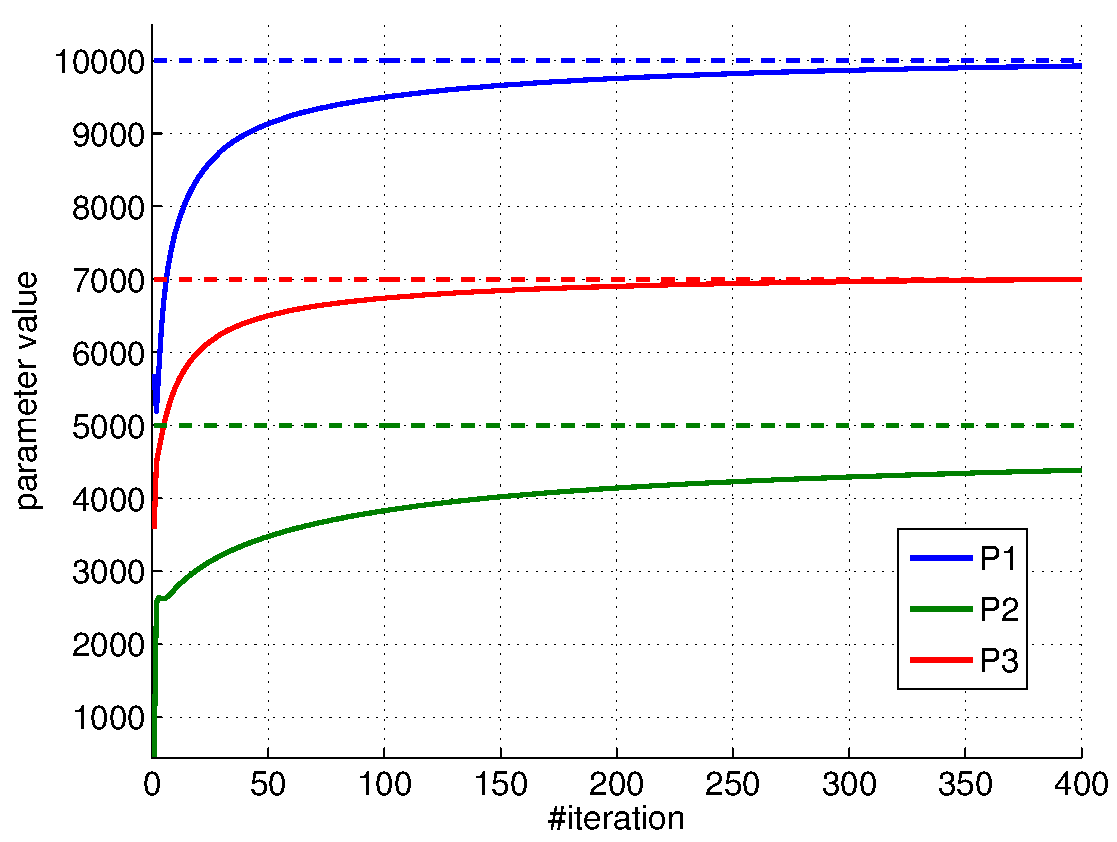
\includegraphics[width=.49\linewidth]{figures/p1_estim.pdf}
\hfill
%\subfigure[]{
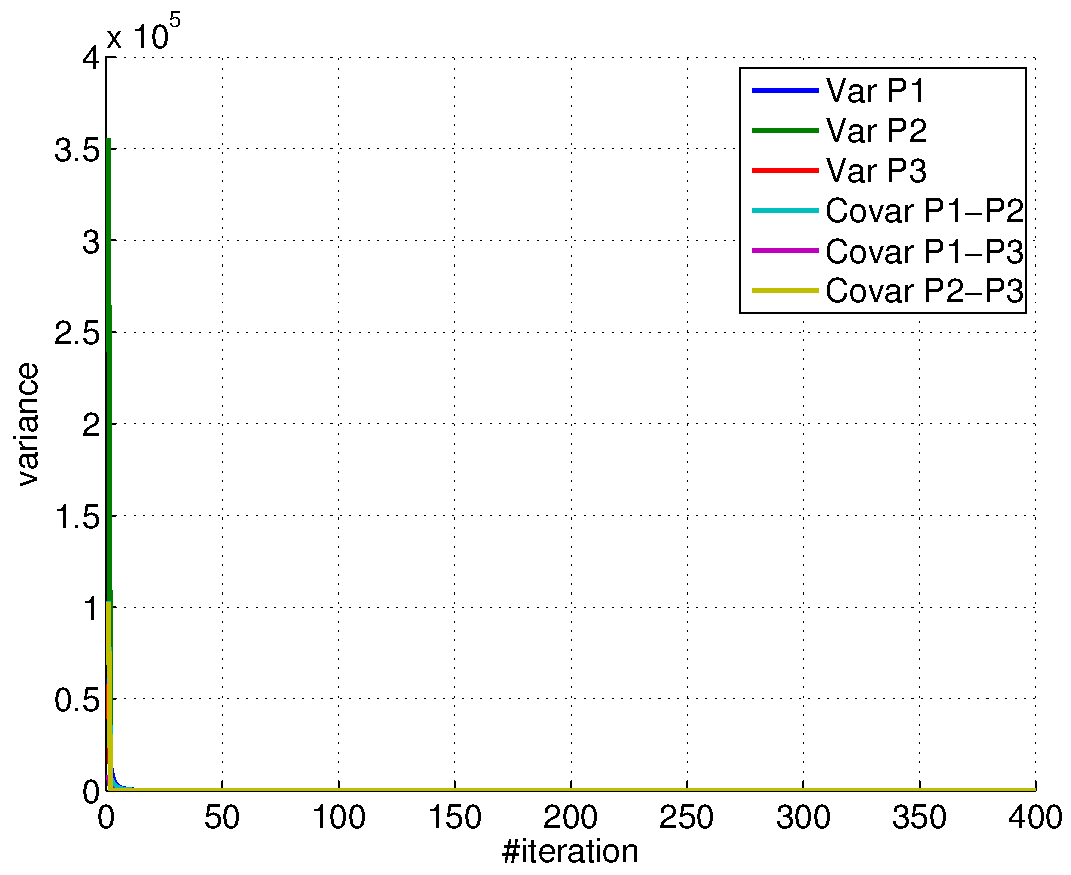
\includegraphics[width=.49\linewidth]{figures/p1_var.pdf}
\caption{Parameters: \texttt{initValue="6000"}, \texttt{stdev="2000"}. Observations: all DoFs (3$\times$number of mesh nodes),
\texttt{observationStdev=1e-4} no noise added. A naive scenario, where everything is known and no uncertainty exists.}
\label{fig:Results1}
\end{center}
\end{figure}


\begin{figure}[h]
\begin{center}
%\subfigure[]{
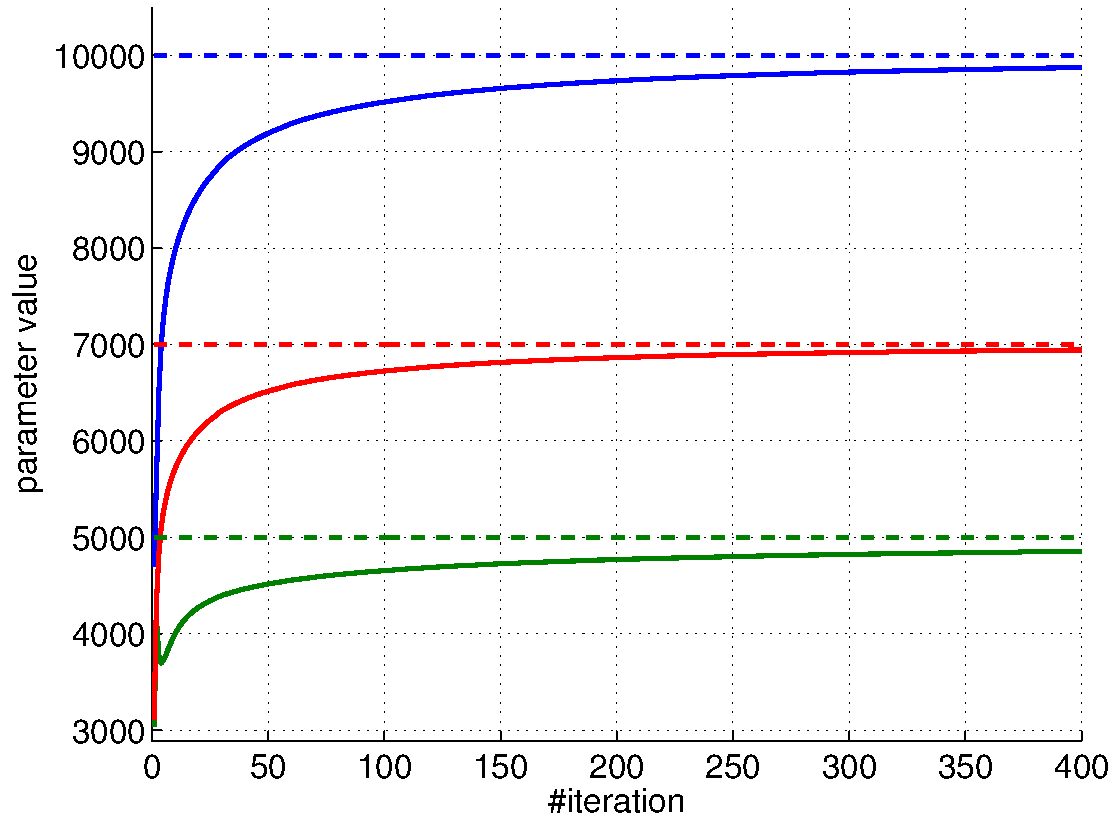
\includegraphics[width=.49\linewidth]{figures/p2_estim.pdf}
\hfill
%\subfigure[]{
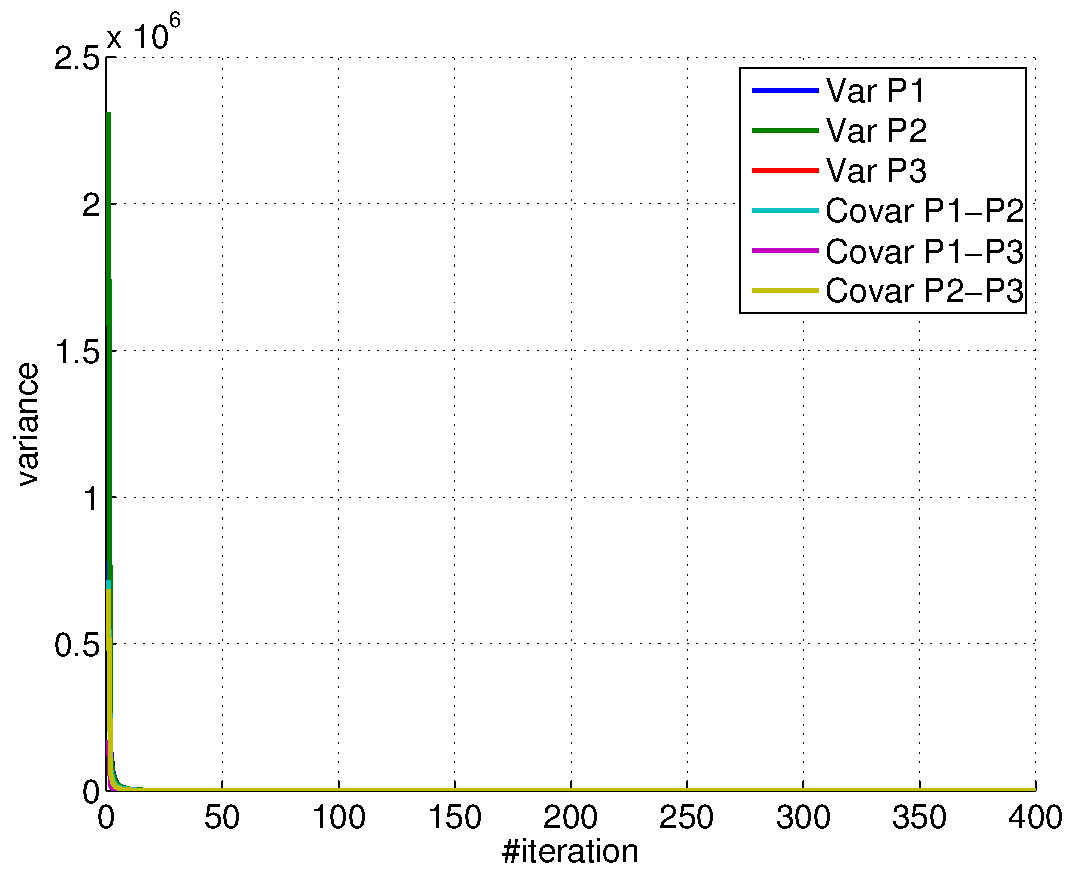
\includegraphics[width=.49\linewidth]{figures/p2_var.pdf}
\caption{Parameters: \texttt{initValue="6000"}, \texttt{stdev="2000"}. Observations: 10 points selected along the centerline,
\texttt{observationStdev=1e-4} no noise added. Still quite naive scenario, where number of observations is limited, but still no uncertainty exists.}
\label{fig:Results1}
\end{center}
\end{figure}



\begin{figure}[h]
\begin{center}
%\subfigure[]{
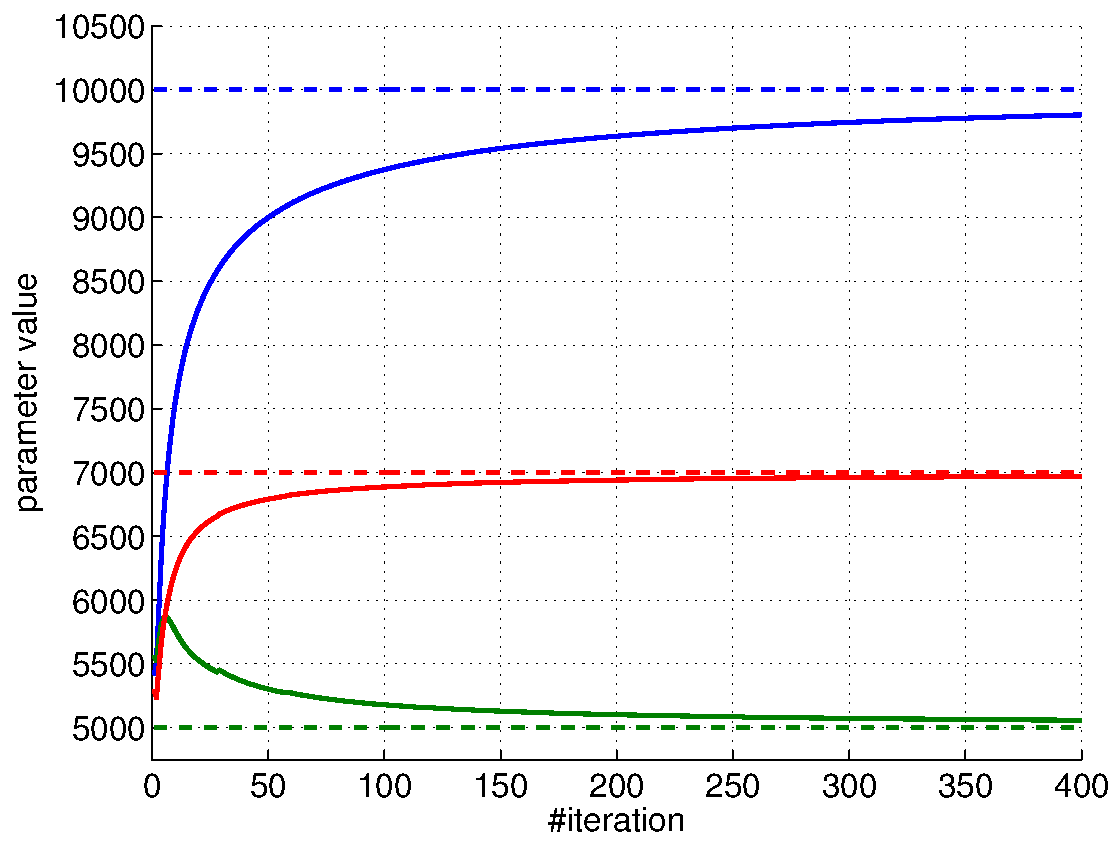
\includegraphics[width=.49\linewidth]{figures/p3_estim.pdf}
\hfill
%\subfigure[]{
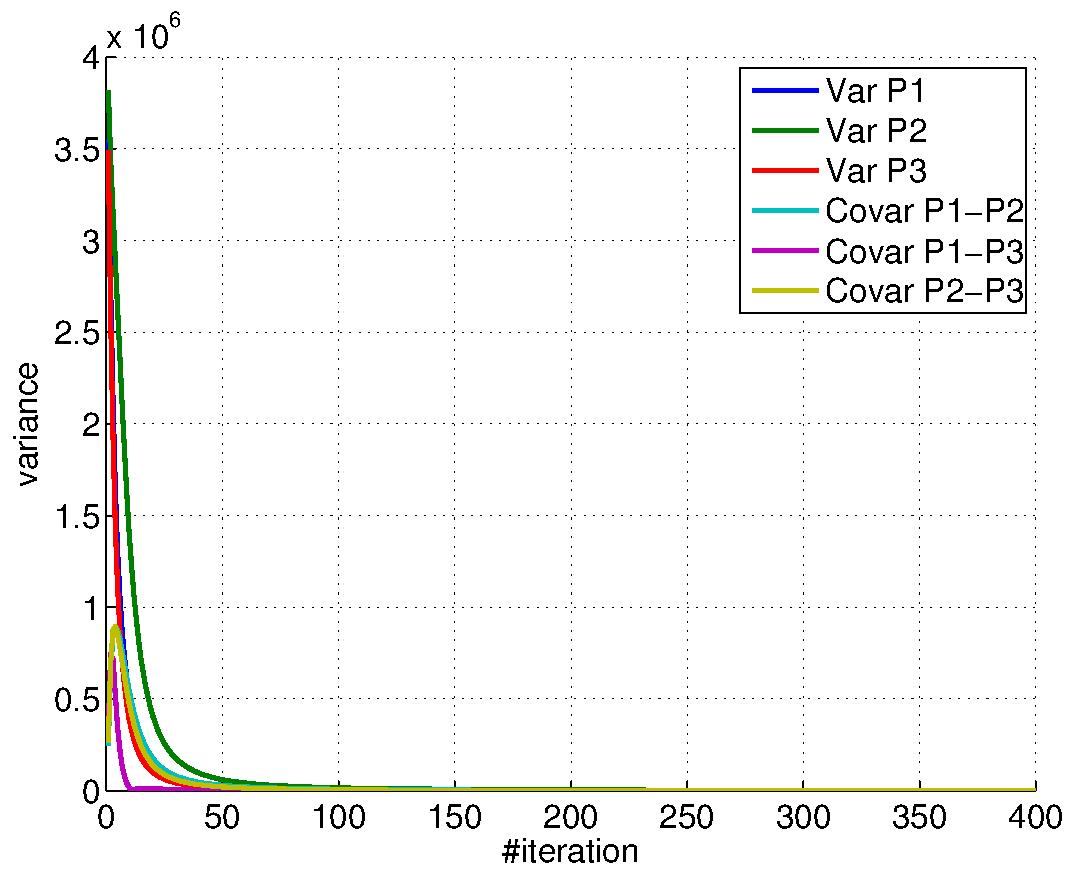
\includegraphics[width=.49\linewidth]{figures/p3_var.pdf}
\caption{Parameters: \texttt{initValue="6000"}, \texttt{stdev="2000"}. Observations: 10 points selected along the centerline,
\texttt{observationStdev=1e-3} no noise added. Although no noise added, we assume uncertainty of 1\,mm for each observation.}
\label{fig:Results1}
\end{center}
\end{figure}



\begin{figure}[h]
\begin{center}
%\subfigure[]{
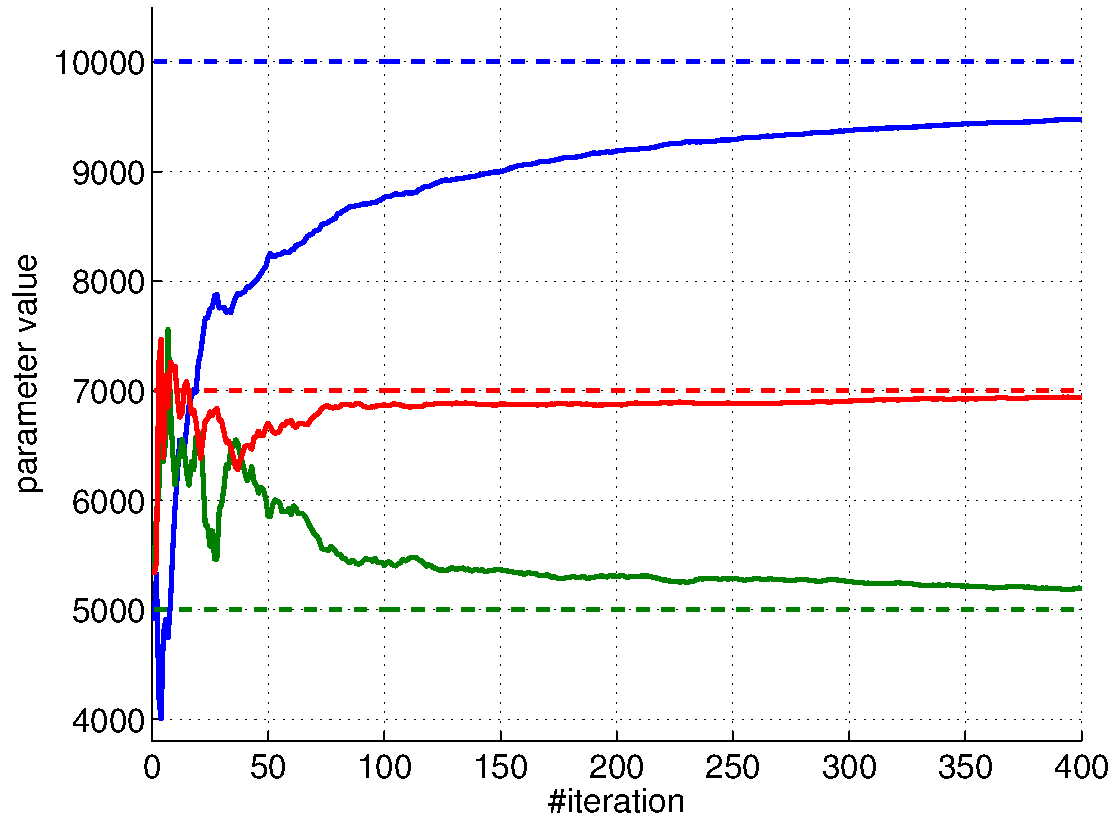
\includegraphics[width=.49\linewidth]{figures/p4_estim.pdf}
\hfill
%\subfigure[]{
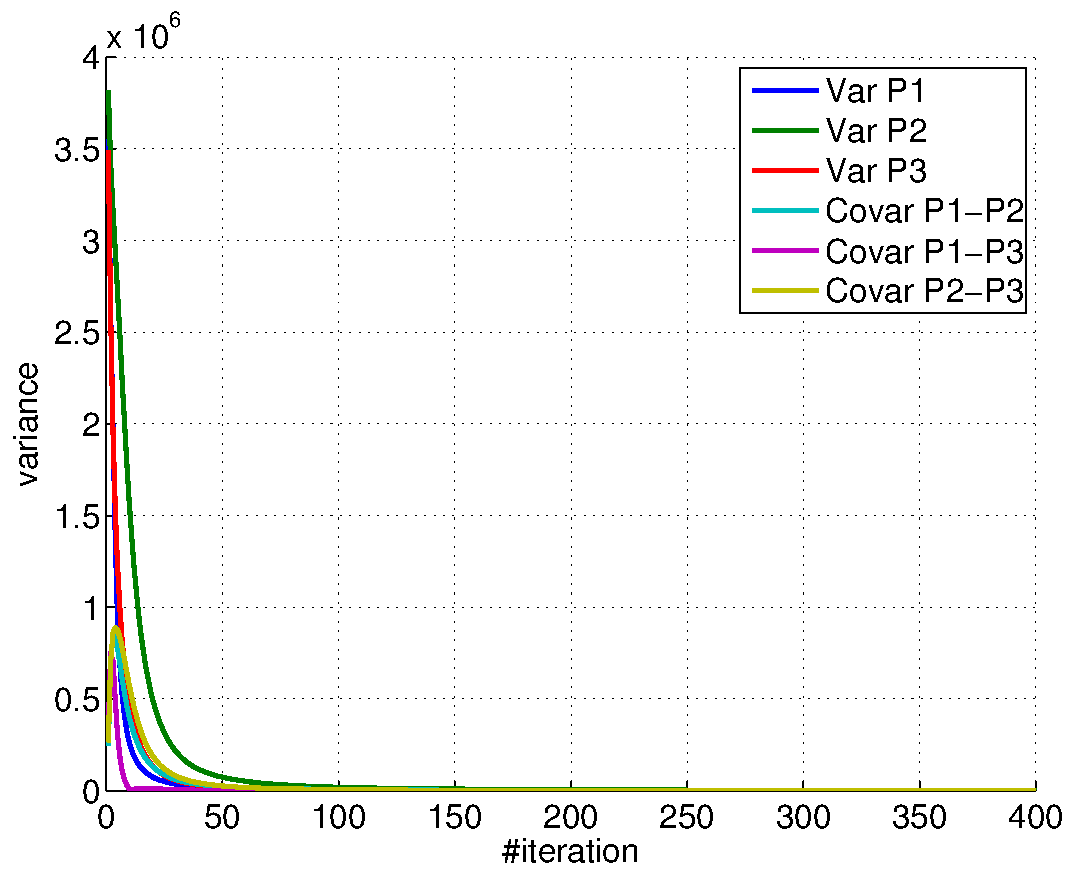
\includegraphics[width=.49\linewidth]{figures/p4_var.pdf}
\caption{Parameters: \texttt{initValue="6000"}, \texttt{stdev="2000"}. Observations: 10 points selected along the centerline,
\texttt{observationStdev=1e-3}, \texttt{noiseStdev=1e-3}. We have a real uncertainty of 1\,mm modeled with white Gaussian noise with standard
deviation of 1\,mm.}
\label{fig:Results1}
\end{center}
\end{figure}



\begin{figure}[h]
\begin{center}
%\subfigure[]{
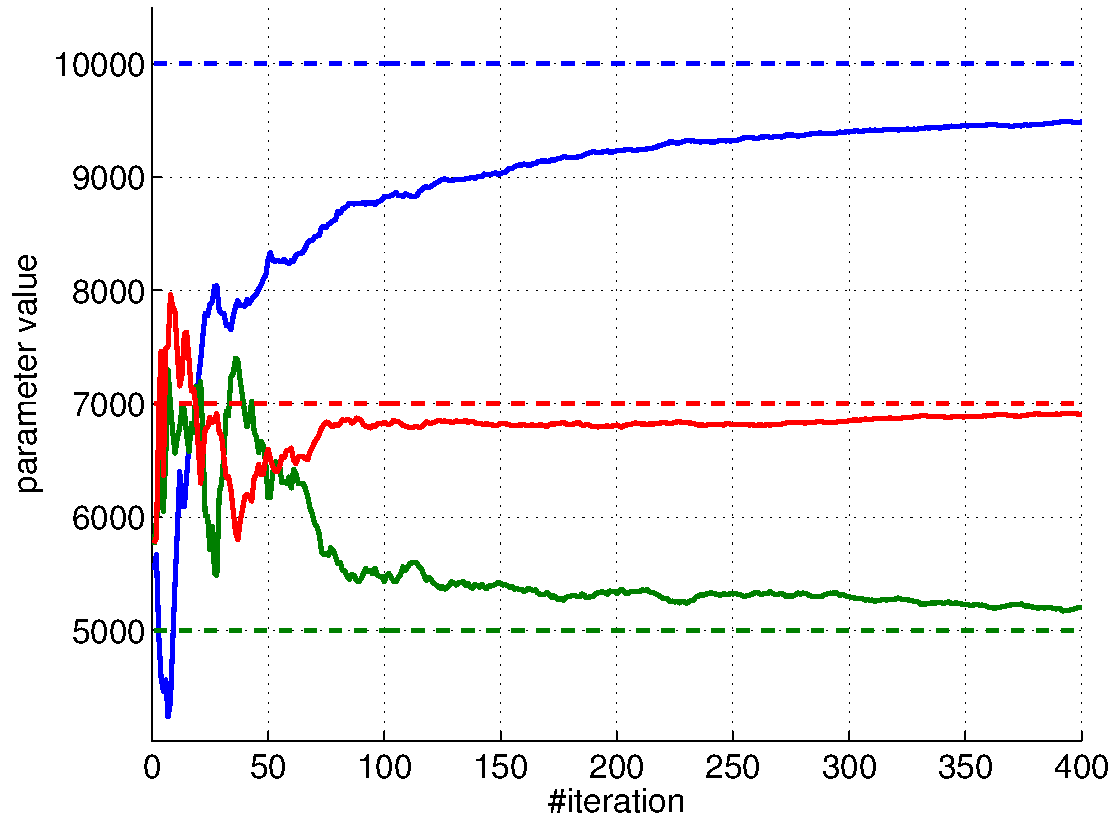
\includegraphics[width=.49\linewidth]{figures/p5_estim.pdf}
\hfill
%\subfigure[]{
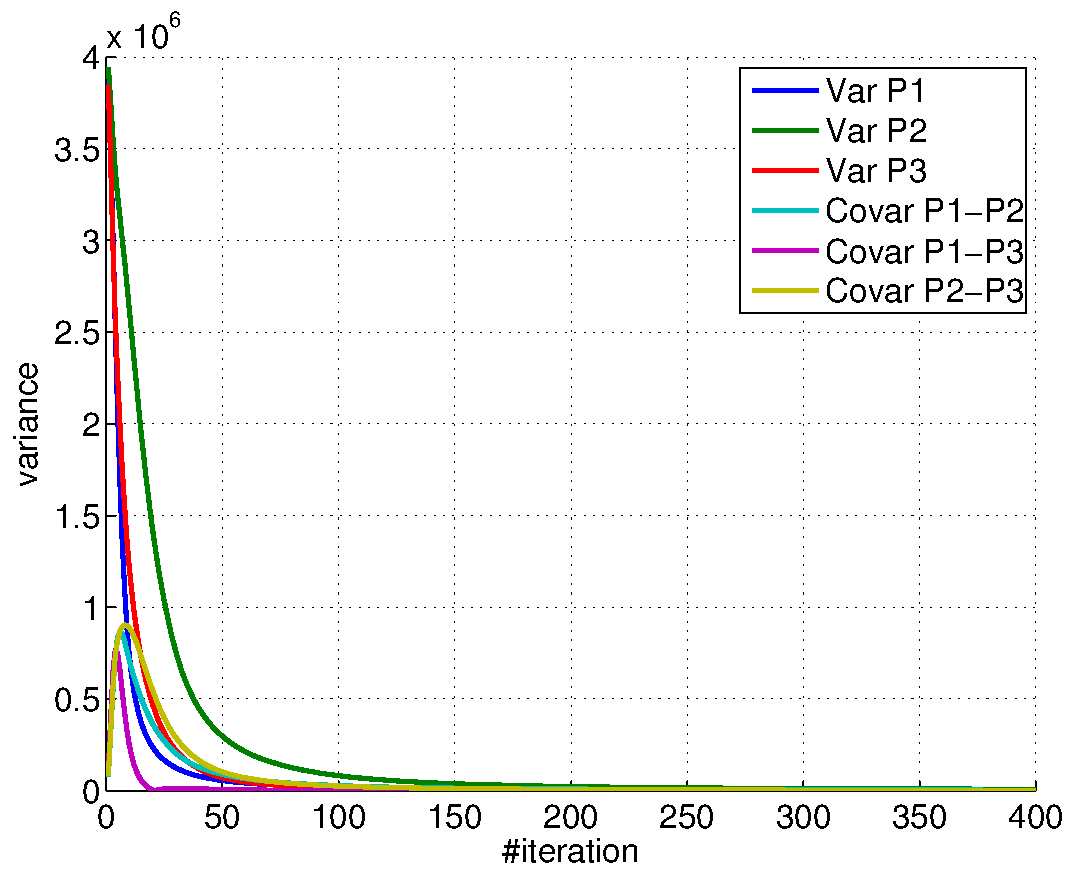
\includegraphics[width=.49\linewidth]{figures/p5_var.pdf}
\caption{Parameters: \texttt{initValue="6000"}, \texttt{stdev="2000"}. Observations: 10 points selected along the centerline,
\texttt{observationStdev=2e-3}, \texttt{noiseStdev=2e-3}. We have a real uncertainty of 2\,mm modeled with white Gaussian noise with standard
deviation of 2\,mm.}
\label{fig:Results1}
\end{center}
\end{figure}



\begin{figure}[h]
\begin{center}
%\subfigure[]{
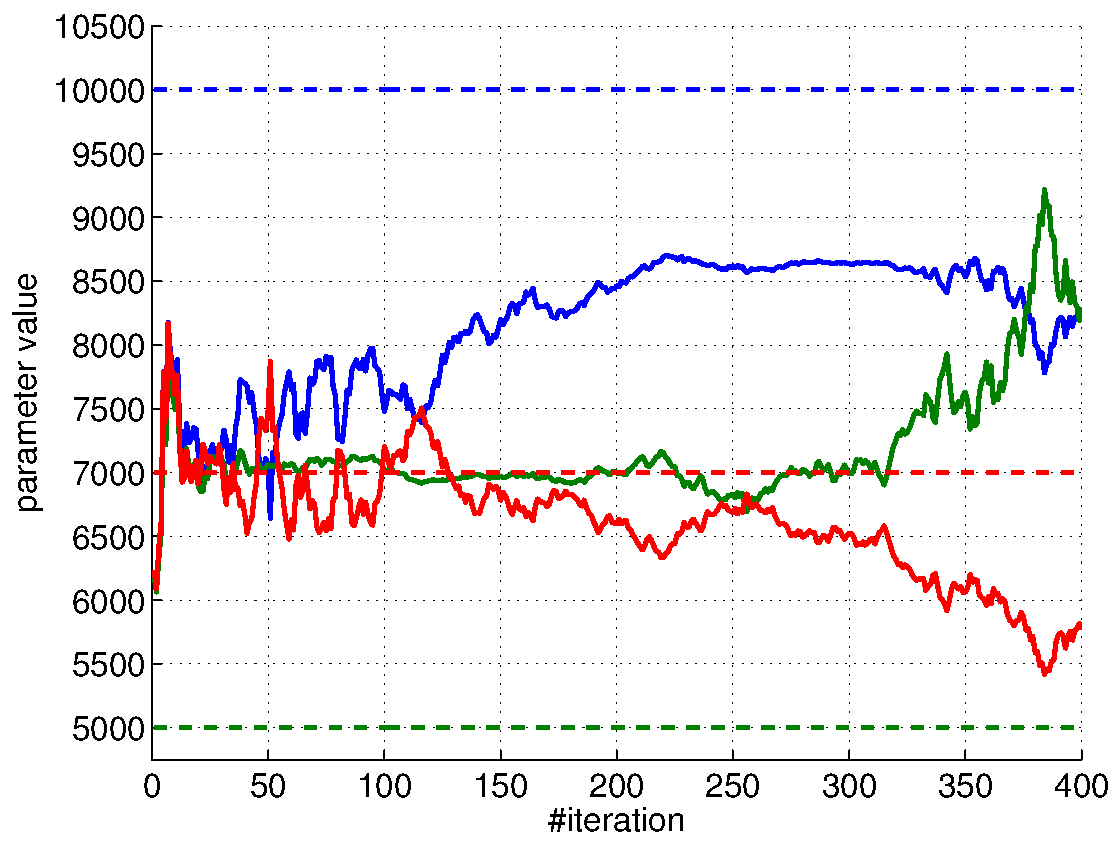
\includegraphics[width=.49\linewidth]{figures/p6_estim.pdf}
\hfill
%\subfigure[]{
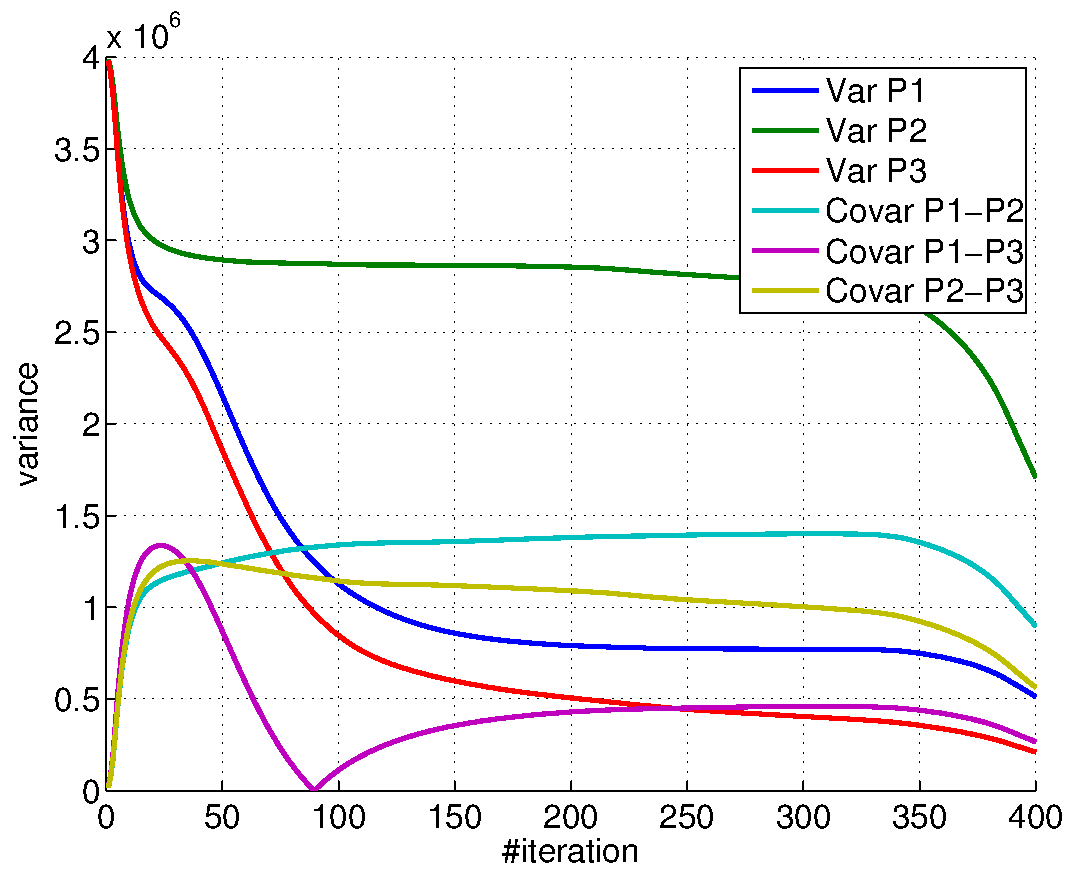
\includegraphics[width=.49\linewidth]{figures/p6_var.pdf}
\caption{Parameters: \texttt{initValue="6000"}, \texttt{stdev="2000"}. Observations: 1 points selected in the middle of the cylinder,
\texttt{observationStdev=2e-3}, \texttt{noiseStdev=2e-3}. An extreme case with fairly limited number of observations (a single point) and a real
uncertainty of 2\,mm modeled with white Gaussian noise with standard deviation of 2\,mm.}
\label{fig:Results1}
\end{center}
\end{figure}




\section{Notes}

\subsection{Static vs. Dynamic}
The graphs in the EX1 were obtained using quasi-static scenario, \ie\ \texttt{StaticSolver} having \texttt{applyIncrementFactor="1"}. Observations:
\begin{itemize}
 \item The result with the \texttt{StaticSolver} depend on \texttt{dt}: the results were obtained with \texttt{dt=0.01s}. Comparable results can be
achieved with \texttt{dt=0.1}, 
 the \svda\ remains stable even for dt of 1\,s.
 \item The stability of the \svda\ seems to depend on the integration scheme, as with \texttt{EulerImplicitSolver} the method seems to be less stable.
The stability depends on \texttt{Rayleigh stiffness}: a behavior comparable to the static behavior is achieved with RS=0.5, the process is stable and
the final approximation is even more precise that in the static case. 
\item With decreasing RS, the DA becomes less stable in the beginning since the change in positions is too fast and so the perturbations becomes
``wild''. 
\end{itemize}






\end{document}
